\chapter{Solución Propuesta}

La solución que se desea brindar es el integramiento de diferentes subsistemas electrónicos que en conjunto permitan resolver el problema
a tratar. Para esto se propone una arquitectura modular compuesta por un sistema de verificación ESD, mecanismos de identificación de usuarios,
monitoreo ambiental, generación de reportes, almacenamiento de registros e interfaz gráfica táctil. La integración de estos subsistemas permitirá
desarrollar una estación inteligente de control ESD de bajo costo orientada a laboratorios de electrónica.

\section{Sistema de verificación ESD}

Para la verificación ESD se hará uso del tester HZR 171 como subsistema principal para la medición de la resistencia eléctrica del usuario. Este
dispositivo es capaz de medir resistencias entre 800 k$\Omega$ y 10 M$\Omega$ con una precisión de $\pm5\%$, lo cual lo hace ideal para mediciones
de pulseras antiestáticas \cite{HZR171}. Sin embargo, no puede ser clasificado como un probador para sistemas de tobilleras debido a que, según los estándares,
el rango de medición requerido se encuentra entre 750 k$\Omega$ y 35 M$\Omega$.

\begin{figure}[H]
        \centering
        
\includegraphics[width=0.45\textwidth]{pics/SP_06.jpg}
        \caption{Probador de pulseras antiestáticas HZR 171, fuente: \cite{HZR171}.}
        \label{fig:HZR171}
\end{figure}

Por lo tanto, se propone utilizar la tarjeta electrónica del HZR 171 como base para dicha medición, integrando las señales $LO$, $OK$ y $HI$ dentro
del sistema general. Además, debido a que este dispositivo requiere una alimentación de 9 VDC \cite{HZR171}, dicha tensión será generada a partir del sistema de
alimentación principal del prototipo.

\section{Sistema de identificación de usuarios}

La identificación de usuarios se realizará mediante dos mecanismos complementarios: reconocimiento facial y lectura de códigos de barras presentes
en los gafetes empresariales.

\subsection{Reconocimiento facial}

Se plantea utilizar el módulo Freenove ESP32-S3 CAM para implementar el reconocimiento facial. Este dispositivo incorpora una cámara y capacidad de
procesamiento suficiente para ejecutar algoritmos livianos de aprendizaje automático, constituyendo una alternativa económica para implementar esta
funcionalidad dentro del proyecto \cite{FreenoveESP32S3CAM}.

\begin{figure}[H]
        \centering
        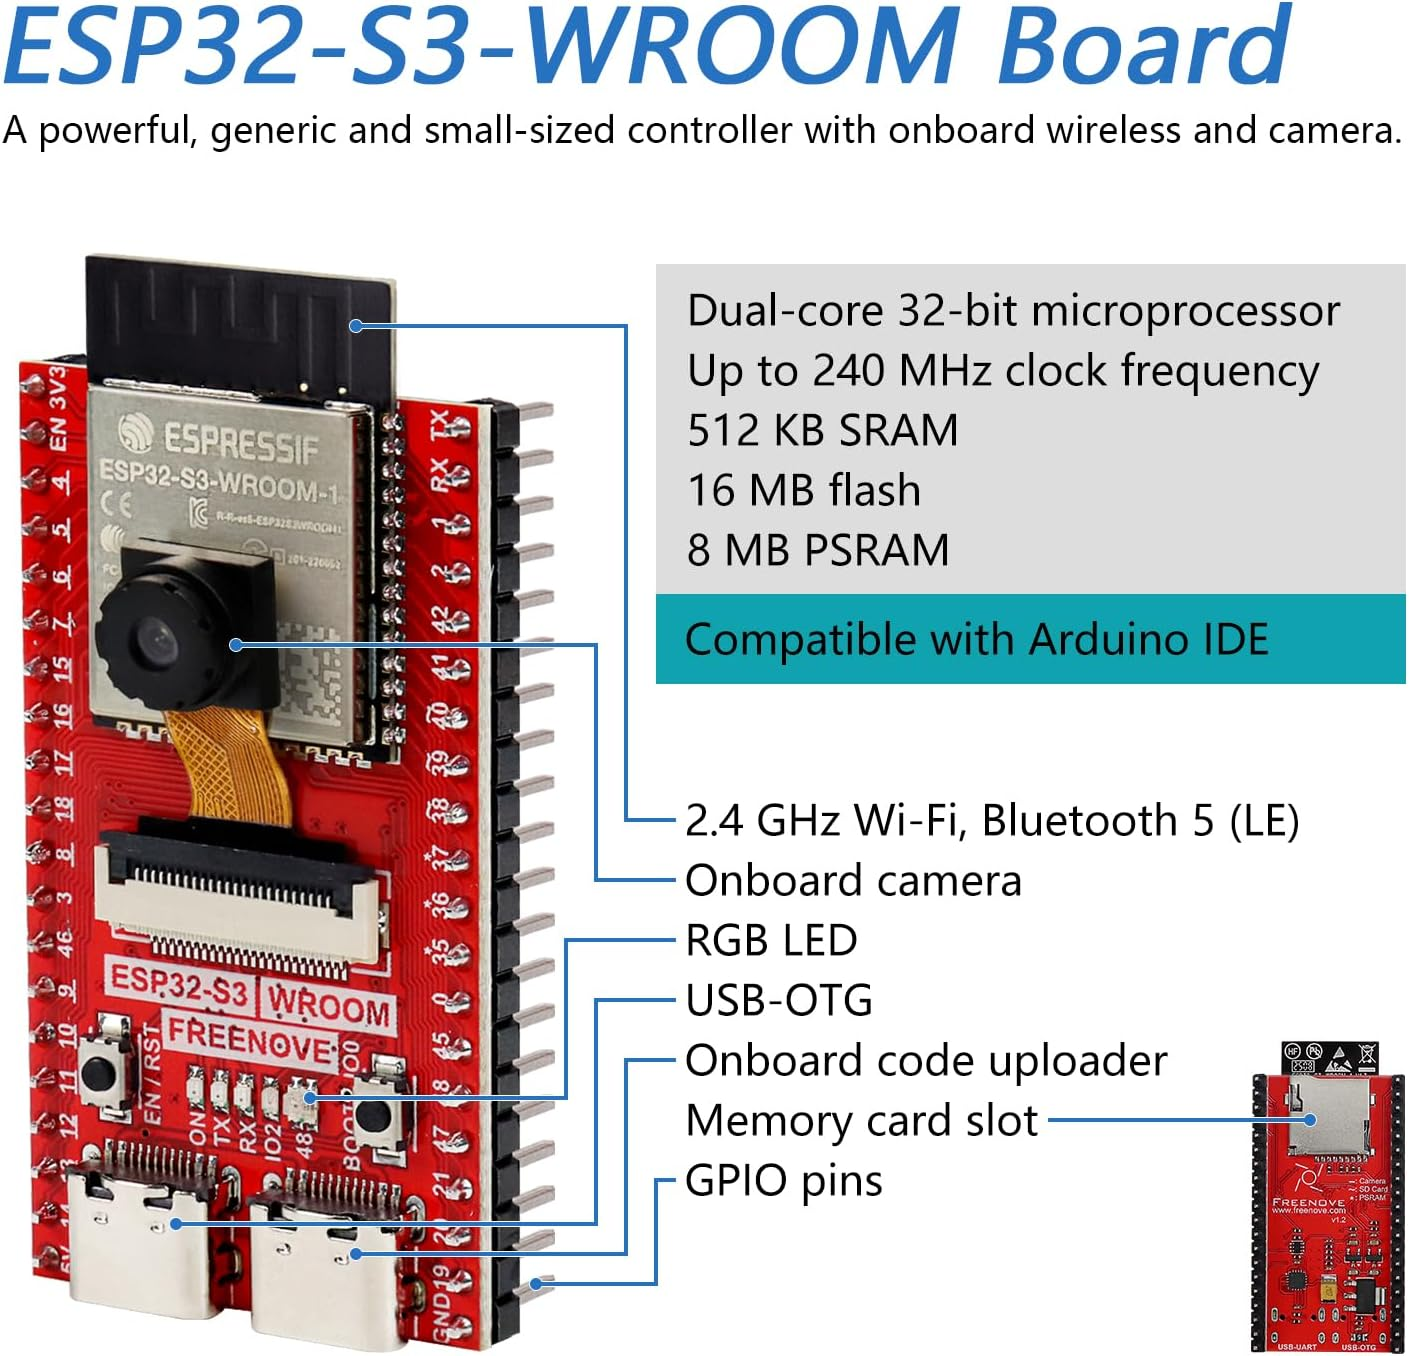
\includegraphics[width=0.45\textwidth]{pics/SP_07.jpg}
        \caption{Módulo Freenove ESP32-S3 CAM utilizado para reconocimiento facial, fuente: \cite{FreenoveESP32S3CAM}.}
        \label{fig:ESP32S3CAM}
\end{figure}

\subsection{Lectura de código de barras}

Para la lectura de códigos de barras se propone utilizar el módulo GM67, el cual emplea comunicación UART, facilitando su integración con el
microcontrolador principal. Además, este dispositivo puede realizar lecturas a varios centímetros de distancia y operar bajo condiciones de
iluminación entre 0 y 100000 LUX, reduciendo la dependencia de la iluminación ambiental del laboratorio \cite{GM67}.

\begin{figure}[H]
        \centering
        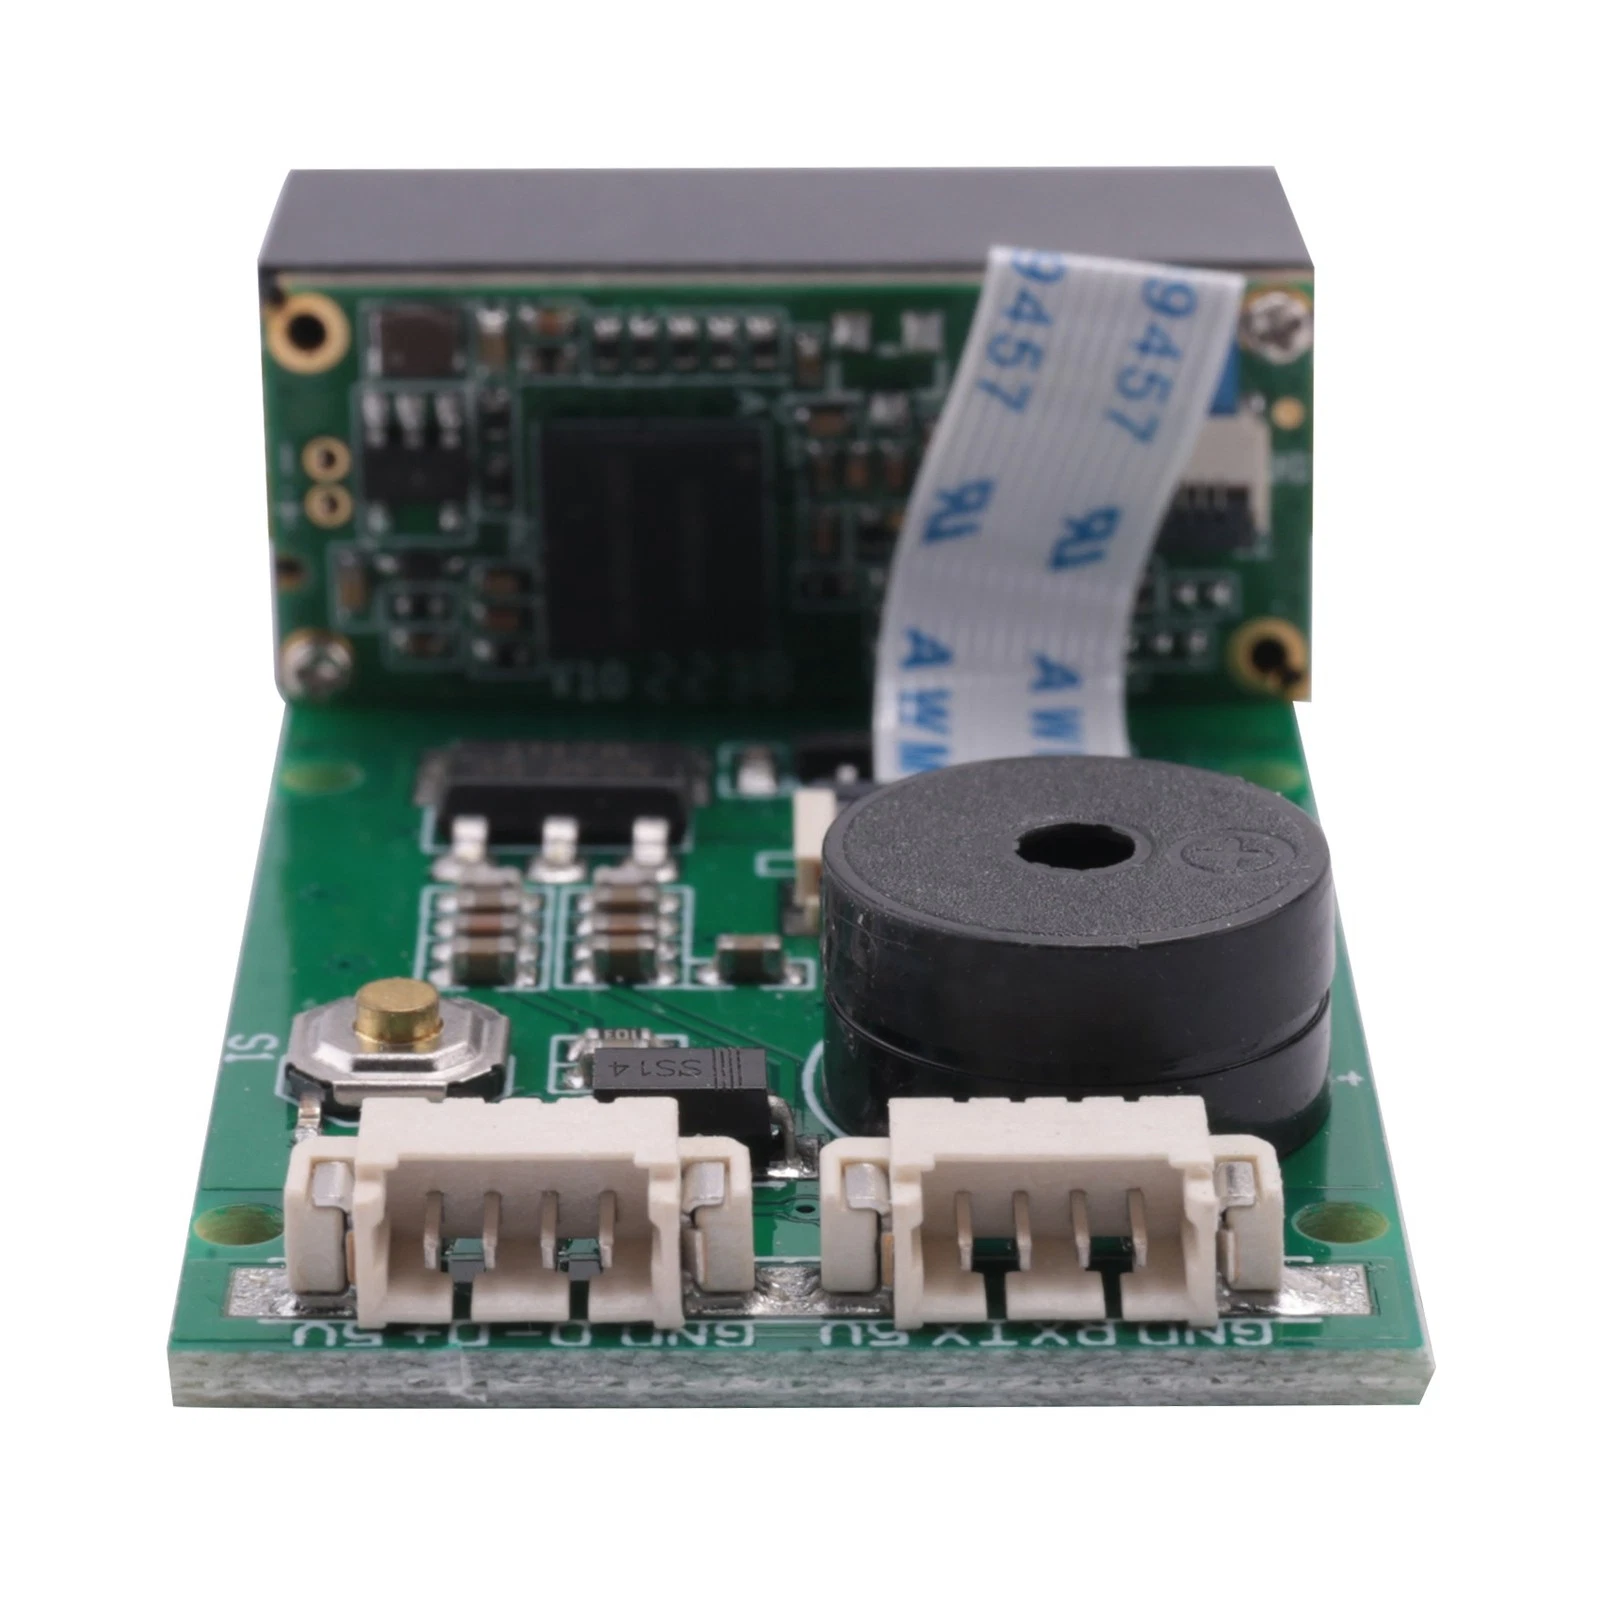
\includegraphics[width=0.45\textwidth]{pics/SP_08.png}
        \caption{Módulo lector de código de barras GM67, fuente: \cite{GM67Ebay}.}
        \label{fig:GM67}
\end{figure}

\section{Sistema de monitoreo ambiental}

Para monitorear las condiciones ambientales se propone utilizar el sensor SHT31-D, dispositivo capaz de medir temperatura y humedad relativa de forma
simultánea. El sensor posee un rango de medición de humedad relativa entre 0 y 100 \% HR con una precisión de $\pm2$ \% HR, mientras que para la
temperatura ofrece un rango entre -40 y 125 $^\circ\mathrm{C}$ con una precisión de $\pm0.3$ $^\circ\mathrm{C}$.

Estas características lo convierten en una alternativa adecuada para registrar las condiciones ambientales durante la ejecución de las pruebas ESD.
El módulo utiliza comunicación I2C, protocolo ampliamente soportado por microcontroladores modernos \cite{SHT31}.

\begin{figure}[H]
        \centering
        
\includegraphics[width=0.45\textwidth]{pics/SP_10.jpg}
        \caption{Sensor de humedad relativa y temperatura SHT31-D, fuente: \cite{SHT31Module}.}
        \label{fig:SHT31}
\end{figure}

\section{Sistema de procesamiento e interfaz de usuario}

\subsection{Interfaz gráfica y almacenamiento}

Para la generación de la interfaz gráfica táctil se propone utilizar el HMI ELECROW ESP32, módulo que incorpora una pantalla táctil de 7 pulgadas,
un microcontrolador ESP32-S3, DAC para reproducción de sonidos, múltiples puertos de comunicación y soporte para memorias microSD.

Estas características permiten implementar una interfaz gráfica capaz de guiar al usuario durante el proceso de prueba, almacenar reportes históricos
y gestionar la información asociada a los mecanismos de identificación implementados. Adicionalmente, el sistema de audio permitirá generar
retroalimentación sonora para mejorar la interacción con el usuario \cite{ElecrowESP32HMIManual}.

\begin{figure}[H]
        \centering
        
\includegraphics[width=0.45\textwidth]{pics/SP_12.jpg}
        \caption{HMI ELECROW ESP32, fuente: \cite{ElecrowESP32HMI7}.}
        \label{fig:HMI}
\end{figure}

\subsection{Controlador principal}

El controlador principal será un ESP32-WROOM-32, encargado de coordinar la comunicación entre los diferentes subsistemas del proyecto. Este
microcontrolador gestionará la interacción con el tester HZR 171, el lector de códigos de barras, el sensor ambiental, el módulo de reconocimiento
facial y la interfaz gráfica.

La selección de este dispositivo se debe a su amplia documentación, bajo costo, disponibilidad de puertos de comunicación y compatibilidad con los
lenguajes de programación utilizados en el desarrollo del proyecto \cite{ESP32WROOM32Datasheet}.

\begin{figure}[H]
        \centering
        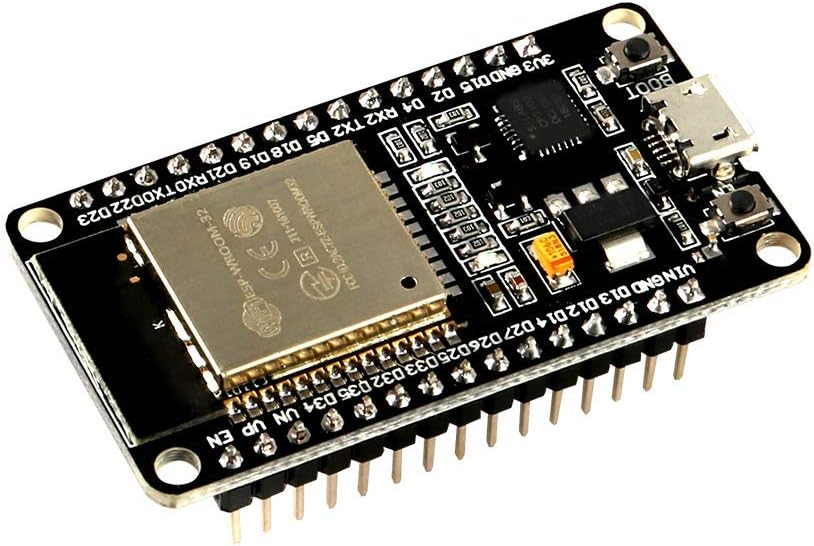
\includegraphics[width=0.45\textwidth]{pics/SP_13.jpg}
        \caption{ESP32-WROOM-32, fuente: \cite{ESP32WROOM32Amazon}.}
        \label{fig:ESP32}
\end{figure}

\section{Sistema de alimentación eléctrica}

\subsection{Alimentación principal}

Para alimentar los módulos electrónicos se requiere una línea de 5 VDC. Debido a que el sistema tendrá interacción eléctrica con el usuario, se busca
reducir al máximo los riesgos asociados a la conexión directa con la red eléctrica.

Por esta razón se propone utilizar un módulo USB-C compatible con el protocolo USB Power Delivery (USB-PD), permitiendo obtener una fuente de baja
tensión y reduciendo significativamente los riesgos eléctricos asociados al prototipo.

\begin{figure}[H]
        \centering
        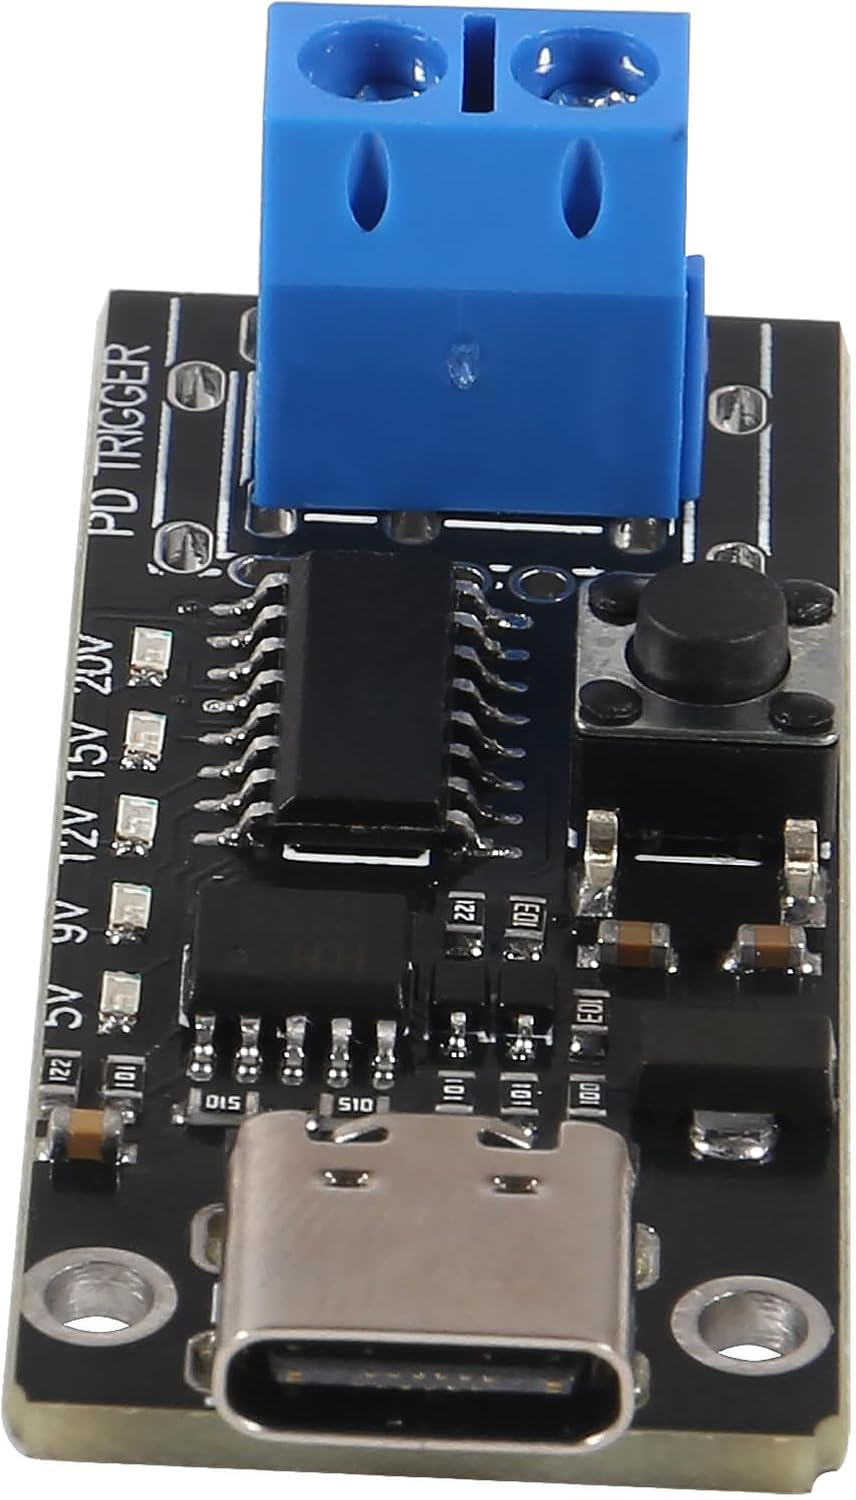
\includegraphics[width=0.25\textwidth]{pics/SP_14.jpg}
        \caption{Módulo USB-C PD, fuente: \cite{AITRIPPDTrigger}.}
        \label{fig:USBPD}
\end{figure}

\subsection{Generación de la tensión para el tester}

El tester HZR 171 requiere una alimentación de 9 VDC, por lo que será necesario incorporar un convertidor elevador de tensión (boost converter).
Para este propósito se selecciona el módulo basado en el circuito integrado XL6019, capaz de generar tensiones de hasta 40 V y suministrar corrientes
de hasta 5 A \cite{XL6019Datasheet}.

\begin{figure}[H]
        \centering
        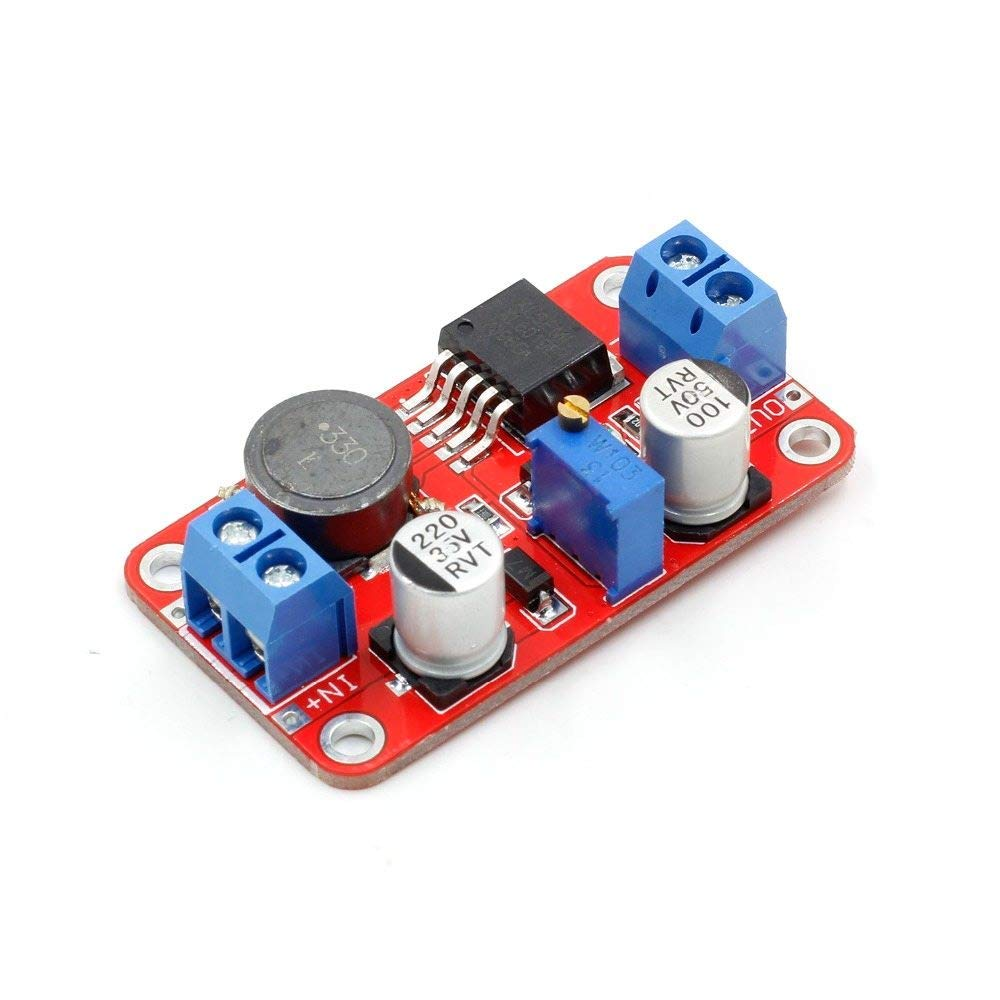
\includegraphics[width=0.45\textwidth]{pics/SP_15.jpg}
        \caption{Módulo basado en el circuito integrado XL6019, fuente: \cite{XL6019BoostModule}.}
        \label{fig:XL6019}
\end{figure}

\section{Integración de los subsistemas}

La integración y conexión de todos los subsistemas descritos anteriormente se muestra en el diagrama de bloques de la Figura~\ref{fig:BloquesSistema}.

\begin{figure}[H]
        \centering
        
\includegraphics[width=0.75\textwidth]{pics/SP_16.png}
        \caption{Diagrama de bloques de la solución propuesta, fuente: elaboración propia.}
        \label{fig:BloquesSistema}
\end{figure}

Para integrar todos los componentes en un único producto se realizará un diseño CAD utilizando Fusion 360 e impresión 3D con PLA como material principal.
Este diseño permitirá alojar los diferentes módulos electrónicos, facilitar el mantenimiento y mejorar la experiencia de uso del sistema.

\begin{figure}[H]
        \centering
        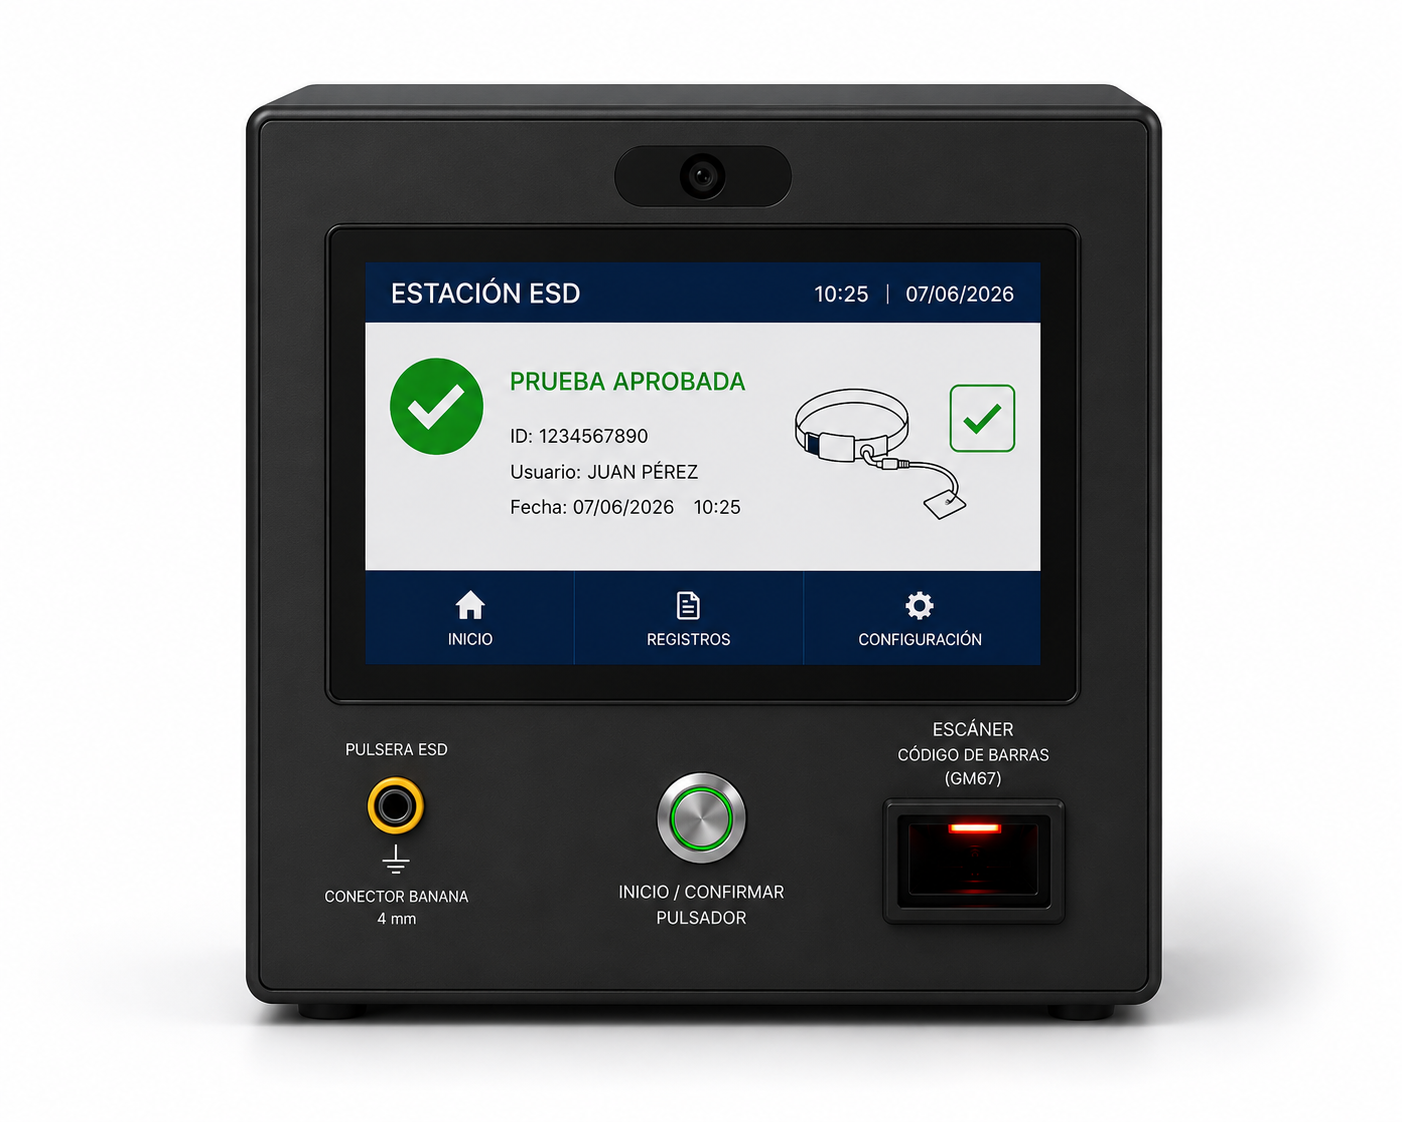
\includegraphics[width=0.75\textwidth]{pics/SP_20.png}
        \caption{Ejemplo conceptual del diseño CAD propuesto para el prototipo, fuente: elaboración propia.}
        \label{fig:CAD}
\end{figure}

La figura anterior muestra un ejemplo conceptual del prototipo entregable propuesto. El diseño final podrá variar durante la etapa de implementación
como resultado de consideraciones mecánicas, eléctricas o de manufactura identificadas durante el desarrollo del proyecto.
